\section{Fremstilling af speckle patterns}

Af de værktøjer der findes til at lave speckle patterns er størstedelen af disse er specialiseret i speckle pattern produktion på mikroskala. I dette afsnit vil der kigges på makroskala, altså værktøjer der kan lave et speckle pattern der kan ses med det blotte øje. Dette betyder prikker med en diameter pr. prik på 0,1mm og over.

\subsection{Stempel og stempelrulle} To værktøjer til speckle pattern produktion er stemplet og stempelrullen. De er let tilgængelige, da de kan købes mange steder, og kun kræver blæk at bruge. De har en større engangsbetaling da det er et specielt værktøj, der kun bruges til speckle pattern produktion. Et sæt med 6 stempler, 6 ruller og noget blæk koster 2350\$ ($\simeq$ 16.700 DKK, d. (25/2-25)) hos Correlated Solutions \parencite{CorrelatedSolutionsVICCorrelation}. Disse værktøjer er lavet til at overføre prikker, ved at de bliver dyppet i maling, som de herefter påfører på en flad overflade. Da mønstret på disse to er identiske fra et tryk til et andet, vil dette give en god genskabelighed og fjerne usikkerheder i forhold til trykmetoden fra forsøg til forsøg. Problemet med disse metoder er at hvert stempel kun skaber mønstrer i ét bestemt størrelsesforhold, hvor der i andre forskellige størrelsesforhold skal bruges større eller mindre prikker, for at ramme 3-7 pixels pr. prik som er defineret i afsnit \ref{Speckle pattern} \parencite{Dong2017ACorrelation}. De størrelser der kommer i sættet fra Correlated Solutions, har stempelruller med prikdiametre fra 0,18mm til 5,08mm, hvilket ved 1920:1080 opløsning, vil give en FOV fra 4,3cm til 325cm \parencite{CorrelatedSolutionsVICCorrelation}. Dette er en høj skalerbarhed, og kan dermed bruges i mange forskellige tilfælde, selvom det er forholdsvist dyrt, at opnå disse flere stempler \parencite{Dong2017ACorrelation}.
\begin{figure}[H]
    \centering
    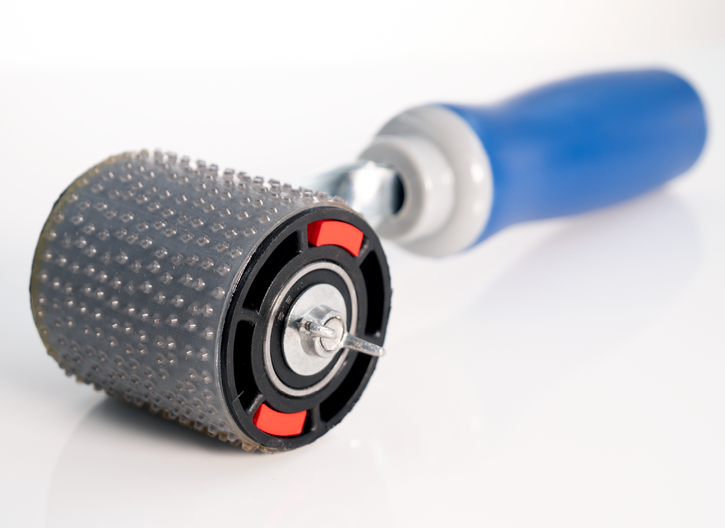
\includegraphics[width=0.4\linewidth]{Sections/2 Problemanalyse/Media/Roller.png}
    \caption{En stempelrulle fra \cite{CorrelatedSolutionsVICCorrelation}}
    \label{Stempelrulle}
\end{figure}

\subsection{Tusch og andre skriveinstrumenter} Et andet instrument der er nemt at anskaffe, er skriveinstrumenter såsom tuscher, kuglepenne og andet der kan påføre farve fra en spids. Her bliver der overført et speckle pattern manuelt ved at sætte prikker i hånden. Skriveinstrumenter er ikke optimale for overførsel af speckle pattern, fordi de kræver en masse tid at lave. Det er muligt at finde specielle tuscher eller kuglepenne, der er lavet med meget små spidser, så der kan laves prikker med en diameter på 100$\mu m$, som kan bruges i FOV'er helt ned til 2,2cm på langs (med en opløsning på 1920:1080).\parencite{Dong2017ACorrelation}. 

En ting der er godt ved skriveinstrumenterne er, at de skal bruges i hænderne af en person, og dette gør at der vil blive en masse usikkerheder i forhold til hvor prikkerne bliver sat. Dette er godt, da det er med til et skabe et unikt mønster, som gør det nemmere at analysere med et computerprogram, medmindre at der rammes de mindste størrelser som nævnt før, her kan det blive et problem, da usikkerhederne kan medføre at der kommer klatter af ren farve eller andre fejl såsom mere farve end 70\% eller mindre end 50\%, som kan medføre fejlmålinger i DIC, grundet mangel på præcision (\ref{Speckle pattern}). Dette er muligt at undgå, hvis der bruges endnu længere tid på at gøre sine prikpositioner perfekte, som medfører mere tid brugt ved mindre skala. Problemet med skriveredskabsmetoden er også, at det er svært og grænser til umuligt at genskabe det samme mønster, således to forsøg kan vurderes på ens vilkår. Det er også et problem at prikkernes afstand i mellem hinanden kan variere, således at der skabes pletter der er for store, eller områder med for lidt dækning af prikker, så der ikke kan observeres en deformation i de områder (Se figur \ref{SpeckleTusch}) \parencite{HoseinSalmanpour2013PDFWalls}. Som nævnt tidligere er disse nemme at erhverve, og det kommer af at 4 tuscher fra 0,1mm diameter til 0,7mm koster 13\$ ($\simeq$ 90 DKK, d. (6/3-25)). hos Amazon \parencite{STAEDTLER2025Amazon.comTousch}.
\begin{figure}[H]
    \centering
    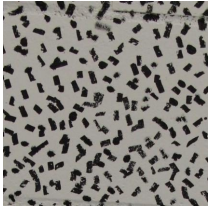
\includegraphics[width=0.4\linewidth]{Sections/2 Problemanalyse/Media/Tusch.png}
    \caption{Speckle pattern med overstregningstusch, som ikke har nok densitet \parencite{HoseinSalmanpour2013PDFWalls}}
    \label{SpeckleTusch}
\end{figure}

\subsection{Spraydåser og Airbrush} En anden metode er spraydåser og airbrusher. Disse producerer speckle patterns på nogenlunde samme måde, nemlig ved at bruge tryk til at affyre maling i en kegleformet udskydning. Spraymetoder er gode til at dække et område hurtigt og forholdsvist tilfældigt, da væsken fra malingen kan samle sig i større klumper, eller blive for sig selv i små pletter. Dette skaber som sagt mere unikke mønstrer. Det bliver til tider et problem, fordi der skabes for store mørke områder eller store samlinger af væske ændrer overfladetykkelsen. En begrænsning med denne metode er også tilfældigheden selv, fordi der aldrig kan genskabes samme mønster som sidste forsøg, og man kan dermed ikke skabe to identiske forsøg med DIC. Derudover er airbrush og spraydåser og begrænsede i, hvor store prikmønstrer de kan skabe. Dette overkommes ved at modificere på afstanden til legemet fra dysen, dysens diameter, tryk i dysen og hvor tyktflydende væsken er. Dette kan bruges til udvide spændet af speckle patterns der kan produceres. Der er stadig en grænse for hvor meget der kan. \parencite{Dong2017ACorrelation, Quino2021SpeckleEndurance}

Spraydåsen og airbrushen er ikke ens, og der er fordele ved at bruge airbrush frem for spraydåser. Her giver airbrushen et mere udspredt speckle pattern, hvor der er en større mængde af større prikker, som giver mere unikke mønstre. Her er problemet med spraydåsen, at der her er større risiko for en stor afvigelse i prikstørrelserne, så der altid vil være prikker der enten er for store eller for små til det ønskede speckle pattern (Se figur \ref{Spraymetode}).\parencite{Crammond2013SpeckleCorrelation}
\begin{figure}[H]
    \centering
    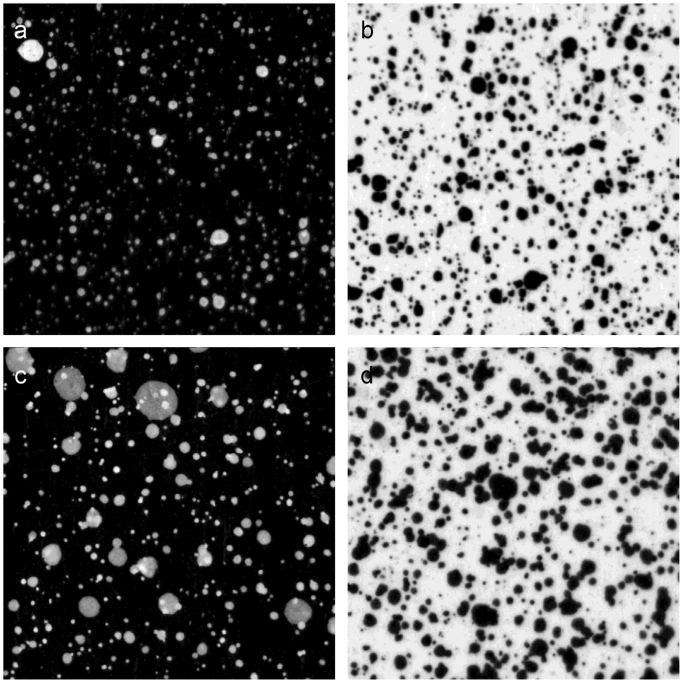
\includegraphics[width=0.5\linewidth]{Sections/2 Problemanalyse/Media/AirvsSpray.png}
    \caption{Speckle patterns med Airbrush og spraydåse. Her er a og b med Airbrush og c og d med Spraydåse \parencite{Crammond2013SpeckleCorrelation}}
    \label{Spraymetode}
\end{figure}

Airbrush det bedre værktøj til speckle pattern produktion og det koster også flere penge, da det har mere specialiserede dele, og kræver en kompressor for at virke.\parencite{Dong2017ACorrelation}) Et billigt airbrushsæt kan købes fra amazon til omkring 600kr.\parencite{TIMBERTECH2025Amazon.comAirbrush}

\subsection{Midlertidig tatovering} En af de sidste speckle pattern metoder der findes i denne skala, er den midlertidige tatovering, som bruges til at overføre et bestemt mønster over på en flade. Dette bruges ved at der genereres et speckle pattern, som laserprintes ind på tatoveringspapiret, og den midlertidige tatovering kan konstrueres som normalt (Se figur \ref{Midlertidigtatovering}). Herefter kan tatoveringen klistres på den ønskede overflade og væde tatoveringen, så blækket overføres og klistrer til den ønskede målte overflade. Dette kan også opskaleres og genskabes med præcist samme mønster igen, da det er printet på tatoveringen. Det koster heller ikke mange penge, og er nemt at få fat i midlertidige tatoveringssæt, det koster fx omkring 75kr. fra Craftelier, at modtage et sæt printbart papir til midlertidige tatoveringer. \parencite{SilhouettePaper} Det kan være en investering at købe en laserprinter, men ellers er dette også en billig løsning.\parencite{Quino2021SpeckleEndurance}

\begin{figure}[H]
    \centering
    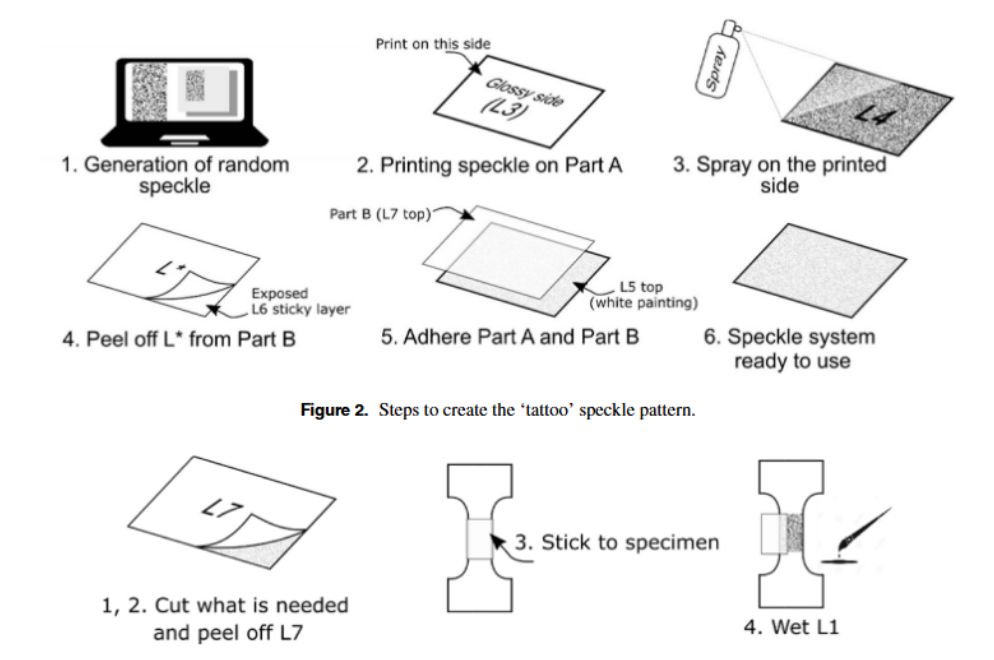
\includegraphics[width=1\linewidth]{Sections/2 Problemanalyse/Media/Temporary tattoo.png}
    \caption{Fremgangsmåde ved påføre af midlertidig tatovering med speckle pattern \parencite{Quino2021SpeckleEndurance}}
    \label{Midlertidigtatovering}
\end{figure}

For at lave en løsning med en robot, er det altså interessant at kunne finde en løsning, der er mere effektiv til at lave speckle patterns end disse løsninger er i forvejen.

\subsection{Optimering} Den mest brugte metode er spraydåsen, altså spraydåser og airbrush \parencite{Dong2017ACorrelation, Quino2021SpeckleEndurance}. Det vil altså være optimalt at kunne lave en løsning, der er mere effektiv end denne løsning. Et af de egenskaber som nogle af de andre værktøjer har, som airbrush og spraydåser mangler, er egenskaben til at kunne genskabe det samme mønster, for at kunne teste på ens vilkår under DIC. Det vil altså være et krav til den ønskede løsning. Derudover er spraymetoden forholdsvist billig, det koster ikke ret mange penge at købe spraydåser, og airbrush koster et rimelig stort engangsbeløb, men ellers kun maling. Det vil altså være et krav, at have en mere priseffektiv løsning, end airbrush og spraydåser repræsenterer i dag.

En af de ting som spraymetoden ikke er god til, er at den er lidt for tilfældige, og store mængder maling kan samle sig på samme sted. Det vil derfor være et krav, at løsningen skal kunne skabe sit mønster igen, og med rimelig præcision således der ikke skabes prikker større end 7 pixels (\ref{Speckle pattern}).